
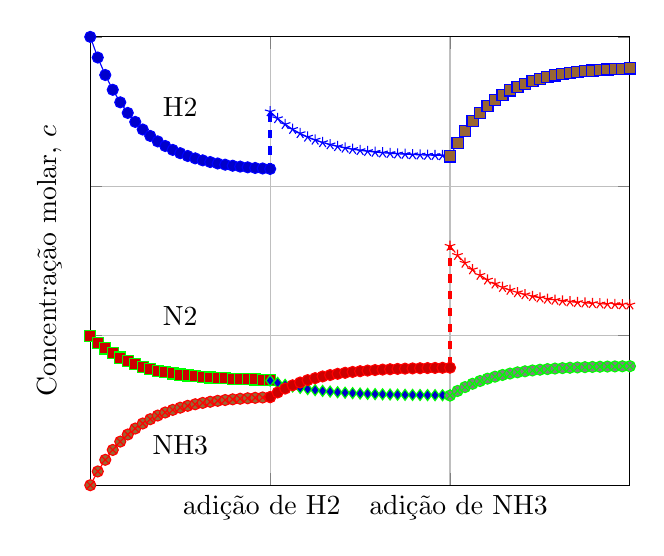
\begin{tikzpicture}
\begin{axis}
    [
        grid = major,
        ylabel = { Concentração molar, $c$ },
        xmin = 0, xmax = 12,
        ymin = 0, ymax = 3,
        xtick = {4, 8},
        xticklabels = { adição de \ce{H2} \;, \; adição de \ce{NH3} },
        yticklabels = \empty,
    ] 
    %%% PRIMEIRA PARTE
    \addplot+ [blue, domain = 0:4]
        { 
            3*exp(-x) + (1-exp(-x))*2.1
        };
    \addplot+ [green, domain = 0:4]
        { 
            1*exp(-x) + (1-exp(-x))*0.7
        };
    \addplot+ [red, domain = 0:4]
        { 
            2*(1-exp(-x)) - (1-exp(-x))*1.4
        };

    %%% SEGUNDA PARTE
    \draw [draw=blue, very thick, dashed]
        (axis cs: 4, 2.1) parabola 
        (axis cs: 4, 2.5);

    \addplot+ [blue, domain = 4:8]
        { 
            2.5*exp(4-x) + (1-exp(4-x))*2.2
        };
    \addplot+ [green, domain = 4:8]
        { 
            0.7*exp(4-x) + (1-exp(4-x))*0.6
        };
    \addplot+ [red, domain = 4:8]
        { 
            2*(1-exp(4-x)) - (1-exp(4-x))*1.8 + 0.59
        };

    %%% TERCEIRA PARTE
    \draw [draw=red, very thick, dashed]
        (axis cs: 8, 0.8) parabola 
        (axis cs: 8, 1.6);

    \addplot+ [blue, domain = 8:12]
        { 
            3*(1-exp(8-x)) - (1-exp(8-x))*2.4 + 2.2
        };
    \addplot+ [green, domain = 8:12]
        { 
            1*(1-exp(8-x)) - (1-exp(8-x))*0.8 + 0.6
        };
    \addplot+ [red, domain = 8:12]
        { 
            1.6*exp(8-x) + (1-exp(8-x))*1.2
        };

    \node [anchor = south] at (axis cs:2,2.4) 
        { \ce{H2} };
    \node [anchor = south] at (axis cs:2,1) 
        { \ce{N2} };
    \node [anchor = north] at (axis cs:2,0.4) 
        { \ce{NH3} };

\end{axis}
\end{tikzpicture}
    